\chapter{Estado del Arte}

En este capítulo se revisan diseños de inversores de características similares a las que debería tener este proyecto, especialmente aquellos que se usan en vehículos de Formula Student. La mayoría de coches eléctricos que compiten en eventos de Formula Student utilizan inversores comerciales. A continuación se describen las opciones más usadas entre los diferentes equipos.

\section{Bamocar PG-D3-700-400}
\begin{figure}[H]
	\centering
	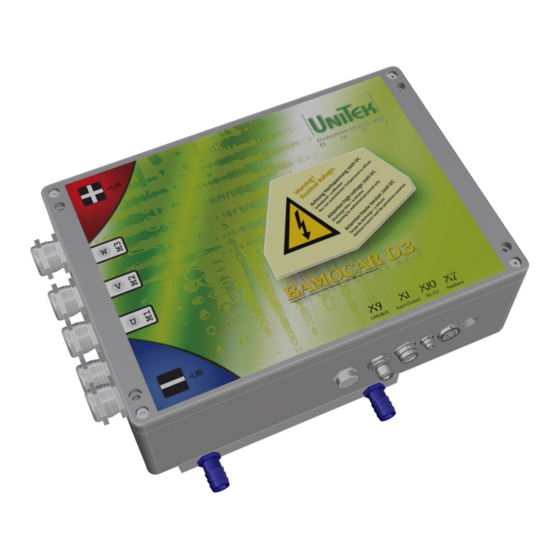
\includegraphics[width=0.7\linewidth]{fig/unitek}
	\caption{Inversor comercial Bamocar PG-D3-700-400 de la empresa alemana Unitek.}
	\label{fig:unitek}
\end{figure}

\begin{itemize}
	\item Fabricante: UniTek GmbH
	\item Potencia máxima: 135 kW
	\item Tensión DC máxima: 700 V
	\item Semiconductores: Si IGBT, módulos \textit{half-bridge}
	\item Capacidad del bus DC: 320 $\mu$F
	\item Frecuencia de conmutación: 16 kHz
	\item Sensor de posición: Encoder incremental, Encoder seno-coseno, Resolver
	\item Control: Control vectorial, consigna de corriente.
\end{itemize}

Esta opción es una de las favoritas para equipos en sus primeros años, ya que no es extremadamente difícil de programar y las puestas en marcha suelen ser rápidas. La desventaja principal es su peso y volumen, ya que están pensados para aplicaciones menos exigentes en cuanto a \textit{packaging} que un monoplaza de competición.

\section{MOBILE DCU 60/60}
\begin{figure}[H]
	\centering
	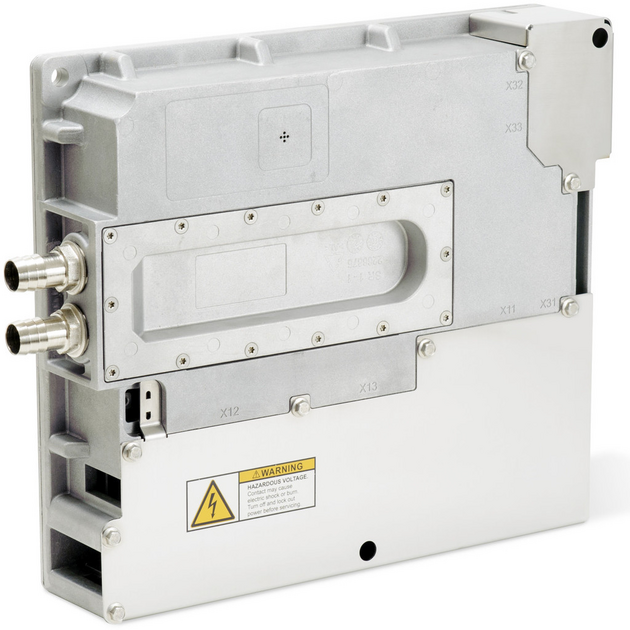
\includegraphics[width=0.7\linewidth]{fig/lenze}
	\caption{Inversor comercial MOBILE DCU 60/60 de la marca suiza Lenze.}
	\label{fig:lenze}
\end{figure}

\begin{itemize}
\item Fabricante: Lenze Shchmidhauser
\item Potencia máxima: 2x60 kW
\item Tensión DC máxima: 848 V
\item Semiconductores: Si IGBT, módulos \textit{six-pack}
\item Capacidad del bus DC: 240 $\mu$F
\item Frecuencia de conmutación: 16 kHz
\item Sensor de posición: Encoder, Resolver
\item Control: Control vectorial, consigna de par y debilitamiento de campo.
\end{itemize}

Este inversor de Lenze es otra de las opciones favoritas de los equipos de Formula Student que montan múltiples motores. Tiene la característica de ser un inversor dual. 

\section{AMK}
\begin{figure}[H]
	\centering
	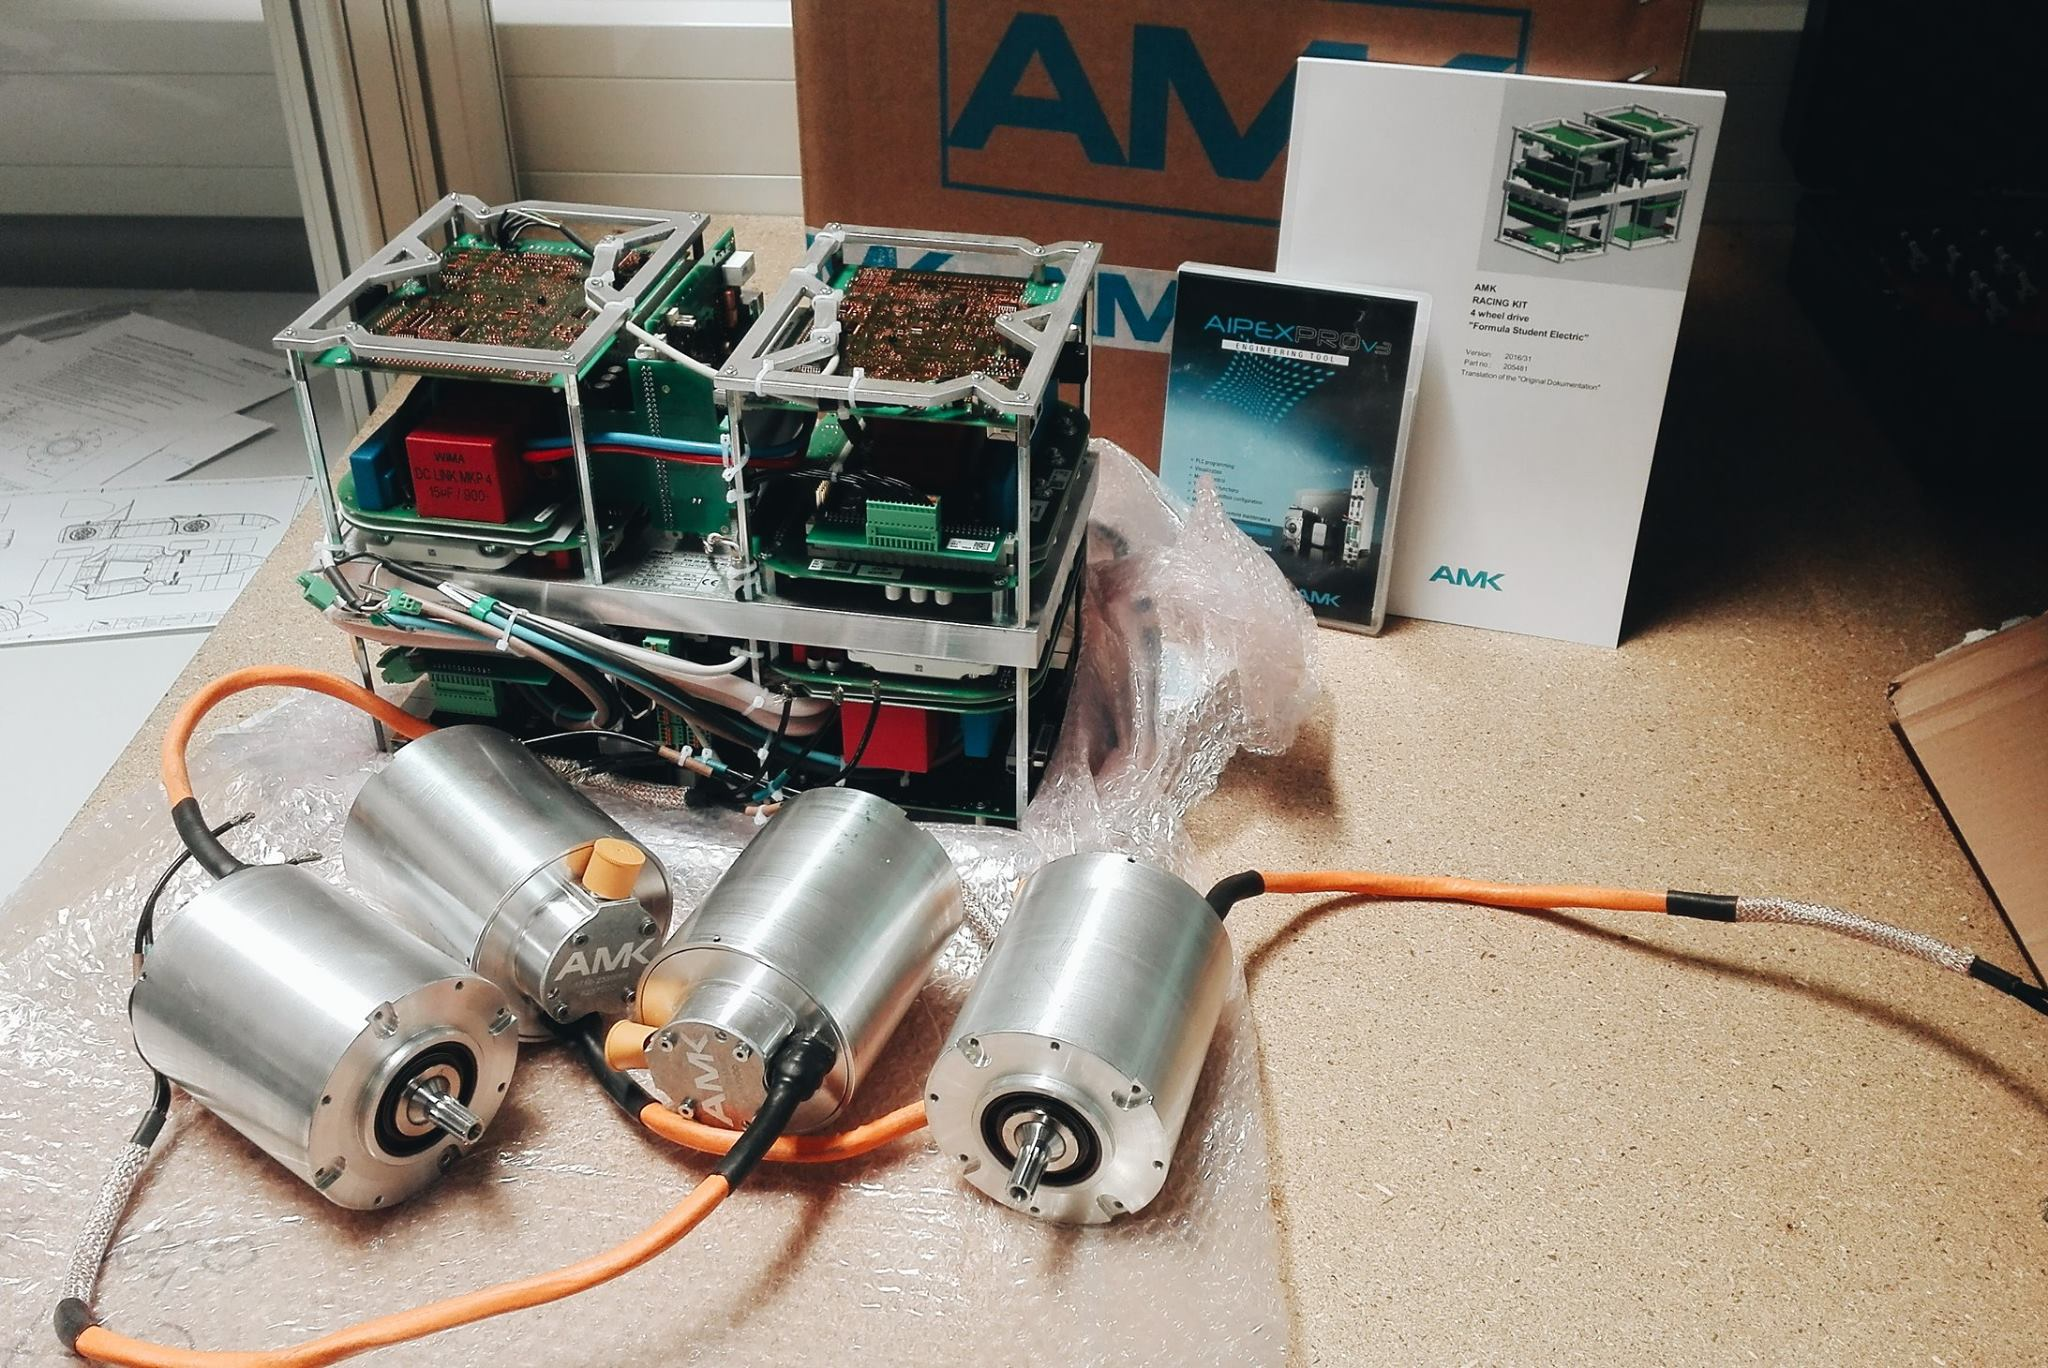
\includegraphics[width=0.7\linewidth]{fig/amk}
	\caption{Inversor comercial AMKASYN KW26-S5-FSE-2Q y motores de la marca alemana AMKmotion GmbH.}
	\label{fig:amk}
\end{figure}

\begin{itemize}
	\item Fabricante: AMKmotion GmbH
	\item Potencia máxima: 2x26 kW
	\item Tensión DC máxima: 720 V
	\item Semiconductores: Si IGBT
	\item Capacidad del bus DC: 1500 $\mu$F
	\item Frecuencia de conmutación: 8 kHz
	\item Sensor de posición: Encoder
	\item Control: Control vectorial, consigna de par y debilitamiento de campo.
\end{itemize}

AMK no solo ofrece este inversor dual si no que también pueden fabricar unos motores eléctricos ideales para su uso junto a estos inversores. Además, tienen la opción de empaquetar dos inversores duales en una sola caja creando un inversor cuádruple, idóneo para monoplazas con tracción integral. Es de lejos la opción favorita para los equipos con motores embebidos en las ruedas, ya es una solución de casi todo el tren de potencia.

\section{CM200}
\begin{figure}[H]
	\centering
	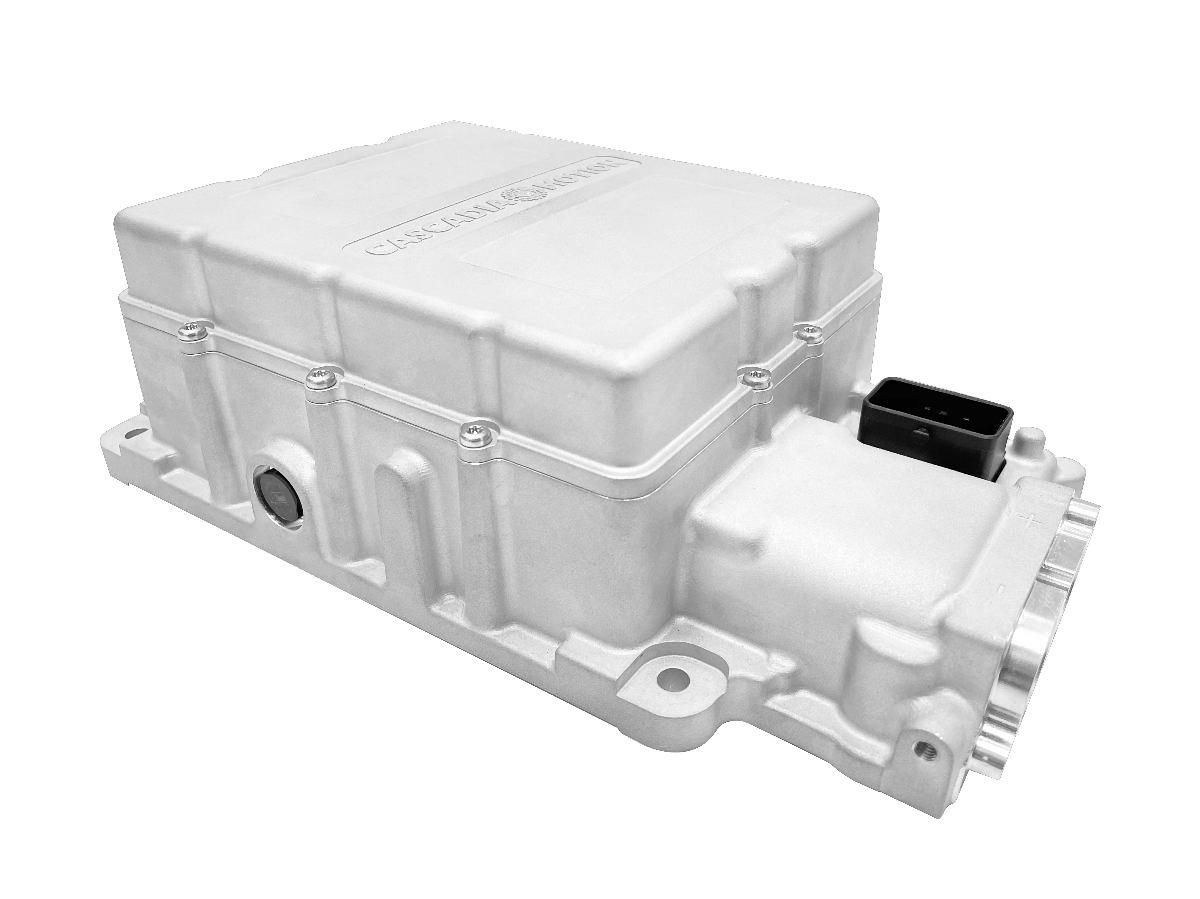
\includegraphics[width=0.7\linewidth]{fig/cascadia}
	\caption{Inversor comercial CM200 de la marca americana Cascadia Motion.}
	\label{fig:cascadia}
\end{figure}

\begin{itemize}
	\item Fabricante: Cascadia Motion
	\item Potencia máxima: 225 kW
	\item Tensión DC máxima: 848 V
	\item Semiconductores: Si IGBT
	\item Capacidad del bus DC: 255 $\mu$F
	\item Frecuencia de conmutación: 16 kHz
	\item Sensor de posición: Encoder, Resolver
	\item Control: Desconocido.
\end{itemize}

Esta empresa ha colaborado históricamente en el desarrollo de inversores para los sistemas híbridos en la Fórmula 1. No hay mucha información al respecto disponible de forma abierta pero se considera un producto interesante.
